\cite{guan2021understanding}, in the context of neural networks, posed the subitization problem one
involving the counting of connected components. To look into this issue, a network was first trained
on random pixel images where the pixel could only have the values of 0 and 1. The 1 was the ``on''
state, with ``0'' being off; the loss was some kind of measure between the number of pixels guessed
and the number of pixels that were actually in the image. It is not clear why this task was chosen,
but the counts that the network output were nearly exactly correct. Afterwards, they counted groups
of pixels as well as shapes. In the former case, pixels were set as on or off randomly, which
created connected components formed by adjacent pixels that happen to be in the ``on'' state. The
more of these neighboring pixels (meaning left, right, top, and bottom pixels) that are ``on'', the
bigger the connected components. The types of shapes that were considered were triangles and
circles.

% ^^^edit2^^^ pointed out formatting issues that (I determined) were caused by using `` and ''
% instead of ", so that was corrected here
The results lead them to claim ``no matter how...the training and test sets [are designed], once the
sizes or types of objects in tests sets become different from training sets, the predictions on test
sets become incorrect''~\cite{guan2021understanding}[§ III]. There were two different scenarios that
they were referring to in this statement. In the first case, how big or how small a single shape
ended up within the same image was independently and identically distributed (i.i.d.). This indeed
had shown problems with the representation learned; see figure \ref{nogeneralizationofshapes}. While
it did predict triangle counts from the same triangle generation parameters successfully, not only
did different sizes throw the network off, but so did different shapes. They suspected that the
average size of a shape being the same between images can result in the network learning that the
number of pixels in the image (not clear if they mean ``on'' or, instead, ``off'' pixels) is the
best feature to regress. As a result, they fixed the size of the shapes within a single image,
and trained from those kinds of samples. They claim that this did not work either, but graph
\textit{b} of figure \ref{nogeneralizationofshapes} actually does show some success, at least for triangles
of vastly smaller sizes. Even for a small number of circles, there does seem to be some sort of
subitization capability. In addition to this evidence, the prediction of the number of connected
components formed by the random pixel-based images were not predicted poorly, either (however, they
point out that the success of this network depended on the requirement that the training set be
similar in possible connected components counts to the test set, which did seem to be the case; see
\cite{guan2021understanding}[figure 5]). They go on to give rationales for the perceived failures of
the network that this author does not necessarily believe to be true given that their networks did
have some amount of success within the definition~\cite{Zhang_2015_CVPR} of subitization.
\begin{figure}[th]
    \begin{center}
        \begin{tabular}{c c}
            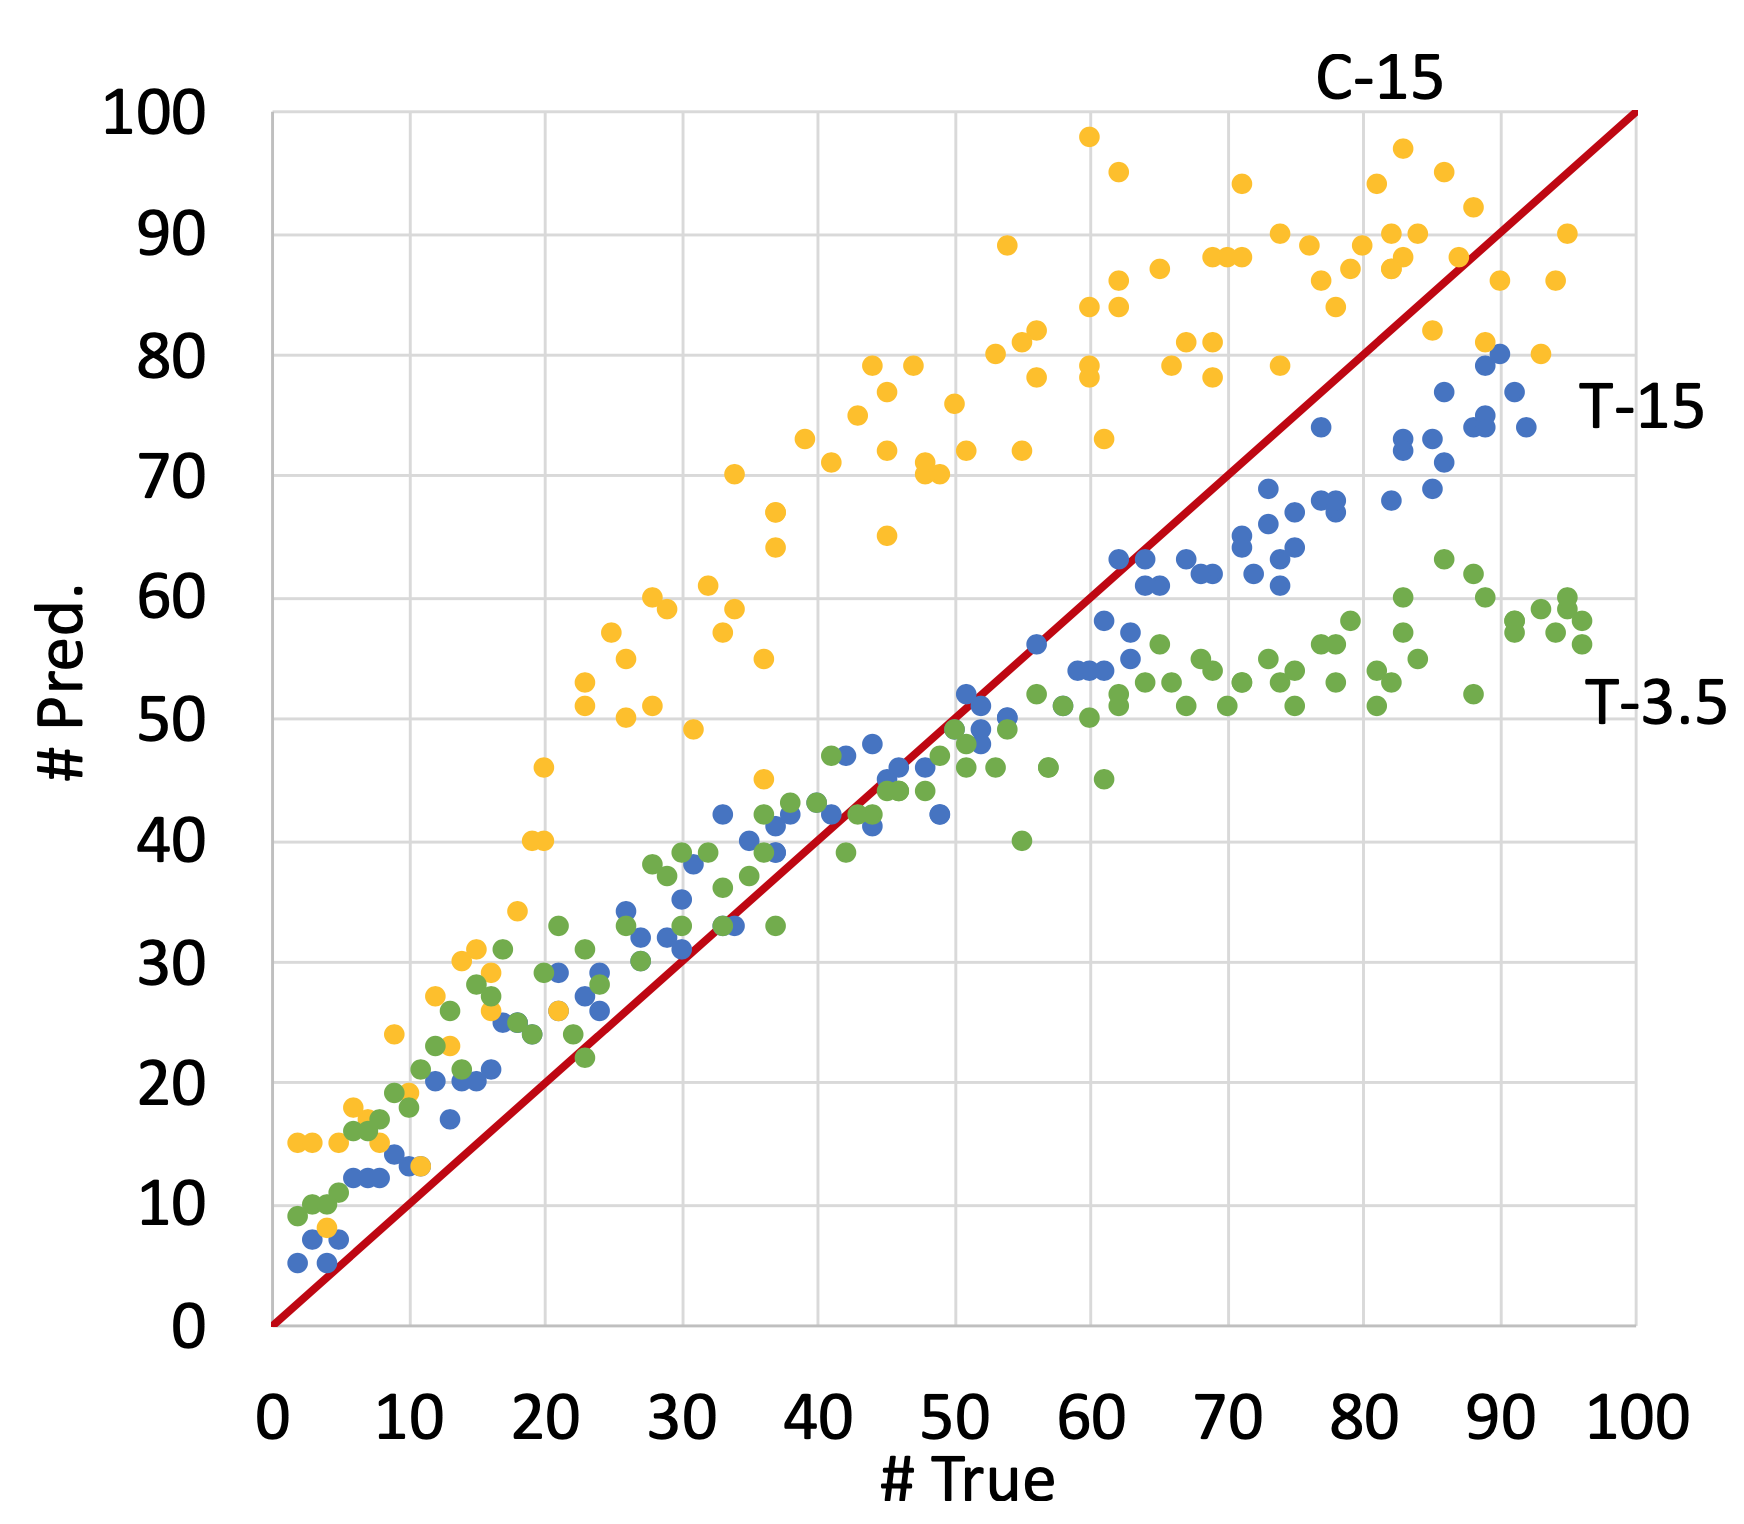
\includegraphics[width = 3in]{Counting/LaTeX/figures/nopropersubitization.png} & 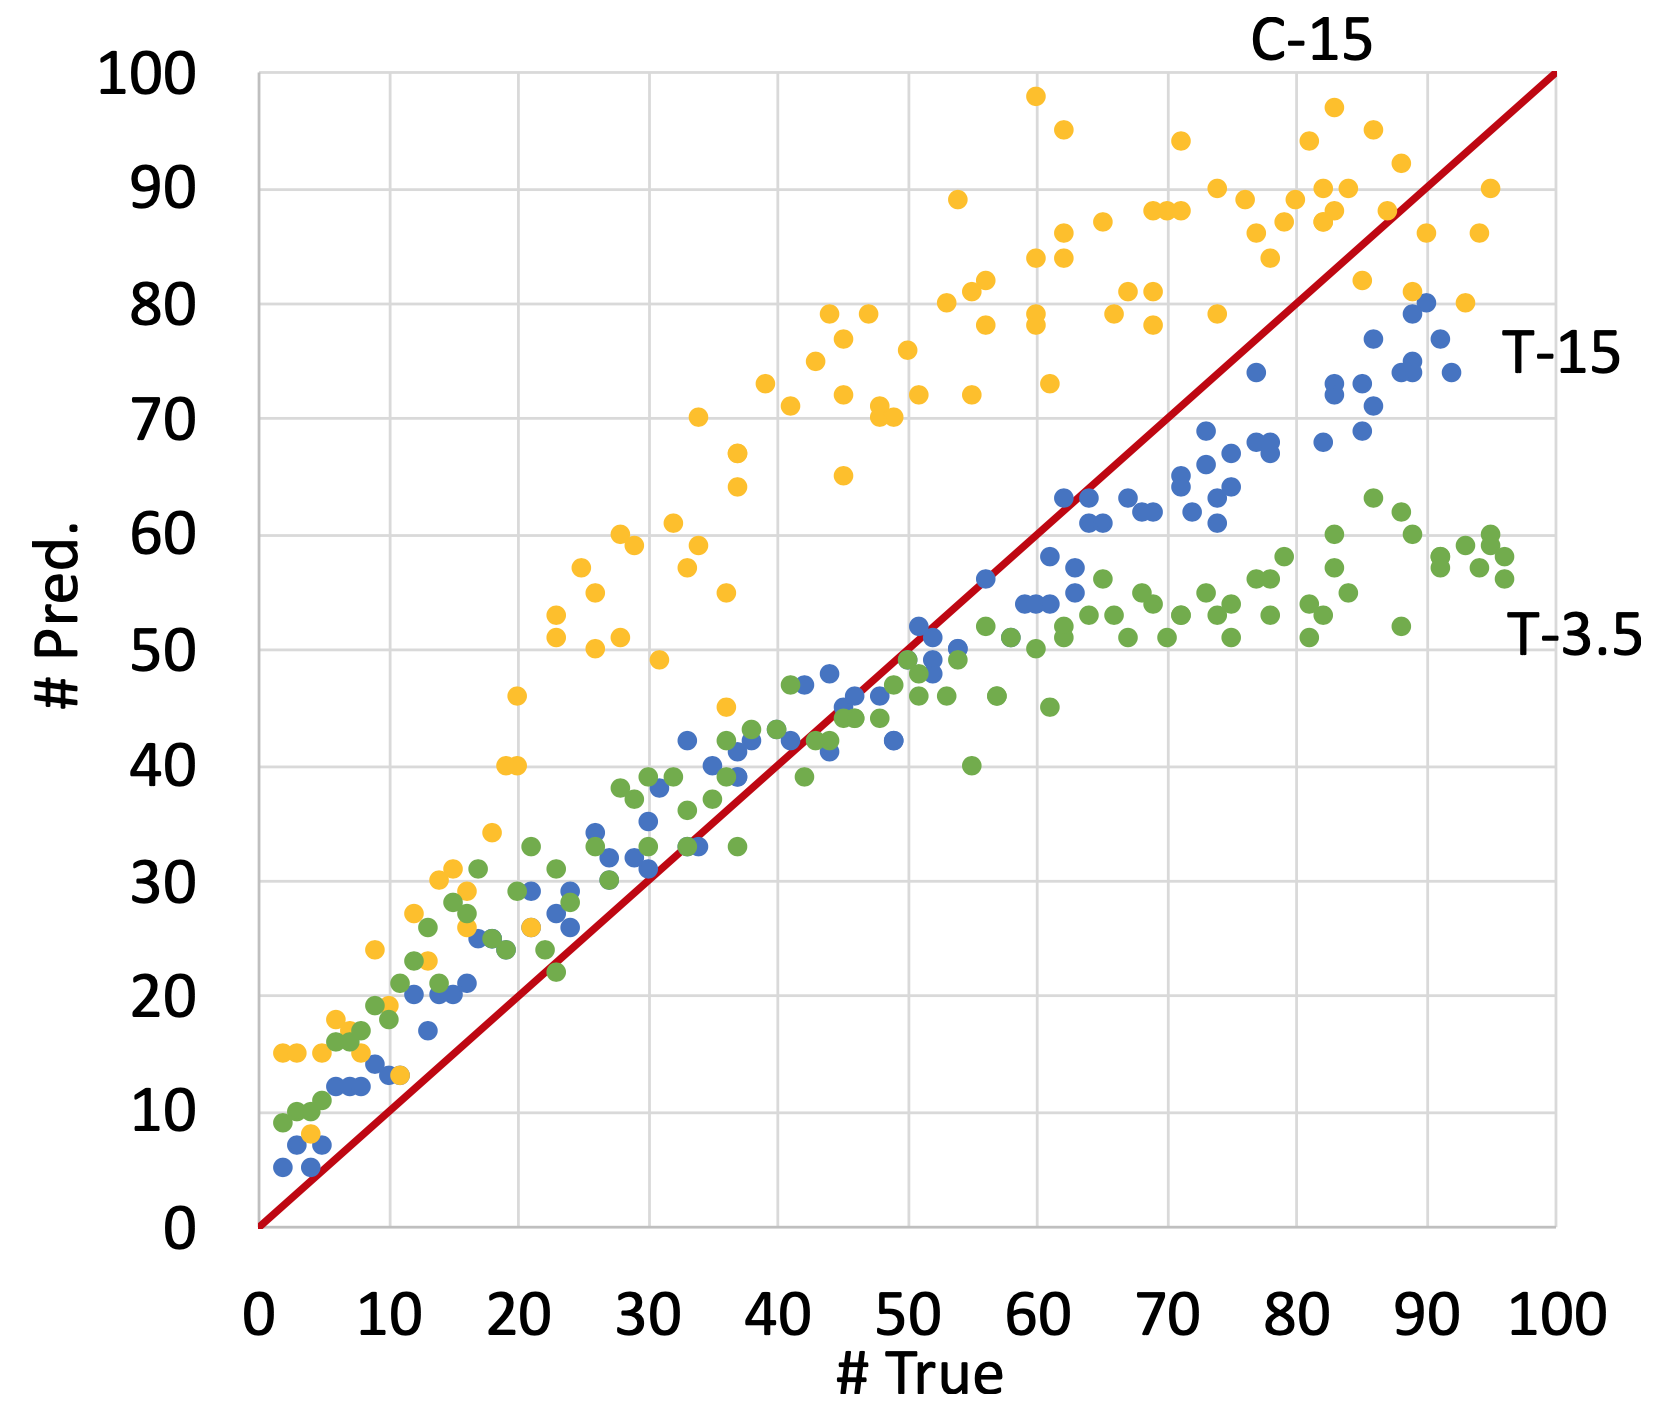
\includegraphics[width = 3in]{Counting/LaTeX/figures/successpartial.png} \\
            \textbf{a}                                                                     & \textbf{b}
        \end{tabular}
        \caption{\cite{guan2021understanding}[figures 4 and 7]'s performance graphs of the model
                 \cite{guan2021understanding} chose. Letters on graph grids refer to the first
                 letter of shapes triangle and circle, and the number after it is some measure of\
                 size.}
    \end{center}
    \label{nogeneralizationofshapes}
\end{figure}

We also refer to and discuss parts of this paper in section \ref{detectionasproofofrepresentation}.
